\documentclass[12pt]{article}

% math typesetting
\usepackage{array, amsmath, amssymb, amsfonts}

% layout control
\usepackage[paper=a4paper,left=25mm,right=25mm,top=20mm,bottom=25mm]{geometry}
\usepackage[onehalfspacing]{setspace}
\setlength{\parskip}{.5em}
\usepackage{rotating}
\usepackage{setspace}
\usepackage{fancyhdr}
\usepackage{parallel}
\usepackage{parcolumns}

% tables, list
\usepackage{tabularx, booktabs, multicol, multirow, longtable}
\usepackage{enumitem}

% graphics stuff
\usepackage[usenames,dvipsnames]{xcolor}
\usepackage{subfig, graphicx, tikz}
\usepackage[space]{grffile} % allows us to specify directories that have spaces
\usepackage[section]{placeins} % prevents floats from moving past a \FloatBarrier or section

\usepackage{float}
\floatstyle{boxed}
\newfloat{textbox}{thp}{lob}
\floatname{textbox}{Box}

% bibliography
\usepackage{natbib}
\bibpunct{(}{)}{;}{a}{}{,}

% font
\usepackage{times}

% misc
\usepackage{enumitem} %no space bewteen item [nosepitem]
% \usepackage{boxedminipage} % floating textbox
\usepackage{setspace}
\onehalfspacing

\usepackage{animate}
\graphicspath{ {../graph/} }
\usepackage[colorlinks=true, allcolors=MidnightBlue, pdftex]{hyperref}

% -------------------- title -------------------- %

\title{Why Best Practice Does Not Work in Practice?\\
        The Political Challenge of Implementation}
\author{Anh Le - IED Intern}
\date{}

\setlength{\headheight}{15pt}
\setlength{\headsep}{20pt}
\pagestyle{fancyplain}

\fancyhf{}

\lhead{\fancyplain{}{Anh Le}}
\chead{\fancyplain{}{The Political Challenge of Implementation}}
\rhead{\fancyplain{}{\today}}
\rfoot{\fancyplain{}{\thepage}}

%%%%%%%%%%%%%%%%%%%% DOCUMENT %%%%%%%%%%%%%%%%%%%%

% \doublespacing

\begin{document}
\maketitle

\begin{abstract}
This paper argues that, while corruption is a classic collective action problem, prevalent anti-corruption initiatives are dominated by a principal-agent framework. Therefore, our current effort does not pay sufficient attention to facilitating collective action---in other words, building the political will to \textit{enforce} reform---leading to widespread implementation gap. The paper discusses two case studies of ADB member countries, Indonesia and Vietnam, to illustrate the importance of political will in anti-corruption efforts. Aware that it is difficult for the ADB to get involved in political matters, the paper proposes the \textit{Indicators and Benchmarks} strategy as a technical approach to solving a political problem. The last section concludes and emphasizes that this strategy is not yet another new tool to directly ``cure'' corruption. Rather, it is a change in mindset, geared towards cultivating an enabling environment for the people to fight against corruption themselves.
\end{abstract}

\newpage
\thispagestyle{plain}
\begin{singlespace}
  \tableofcontents
  \listoffigures
\end{singlespace}
\begin{doublespace}
  \renewcommand{\figurename}{Box}
  \listof{textbox}{List of Boxes}
\end{doublespace}

\section*{Abbreviation}
\begin{tabular}{ll}
ADB & Asian Development Bank \\
BPA & Business Process Analysis \\
CRC & Community Score Card \\
CPI & Corruption Perception Index \\
CPS & Country Partnership Strategy \\
DB & Doing Business \\
DMC & Development Member Country \\
ESCAP & Economic and Social Commission for Asia and the Pacific (United Nations) \\
GACAP II & Second Governance and Anti-corruption Action Plan \\
IB & Indicators and Benchmarks \\
IED & Independent Evaluation Department \\
ITFPM & Integrated Trade Facilitation Performance Monitoring \\
KPK & Corruption Eradication Commission (Indonesia) \\
PCI & Provincial Competitiveness Index (Vietnam)  \\
PETS & Public Expenditure Tracking Survey \\
QSDS & Quantitative Service Delivery Survey \\
RCT & Randomized Controlled Trial \\
RM & Resident Mission \\
RSDD &  Regional and Sustainable Development Department \\
SARD & South Asia Department \\
SASEC & South Asia Sub-regional Economic Cooperation \\
TA & Technical Assistance \\
TCD & Time-Cost-Distance \\
TRS & Time Release Studies \\
WGI & World Governance Index \\
\end{tabular}

\newpage
\section{Introduction} \label{sec:intro}

In the latest \citet{Integrity2012a} report, which ranks countries on their anti-corruption effort, an Asian country stands out remarkably. It boasts an exemplary score of 86.9 on legal framework, higher than Germany's 81.0. It has perfect anti-corruption law, which criminalizes bribery, extortion, and misuse of public assets. Better yet, the country has established a host of supporting institutions, including a national ombudsman protected by law against political interference---something that is left for citizens to desire even in the United States \citep{MinistryofLawandJustice2003}. On top of that, there is an independent agency with the legal mandate to address corruption, whose leader can only be removed by the head of a democratically elected government based on an inquiry by the Supreme Court.

The country in question is India, a place deeply mired for years in corruption. This puzzling mismatch between law and practice is by no means unique to India: China and Mongolia, whose legal frameworks earn a score of 78 and 80, are in the same league with Germany. This pattern extends well beyond Asia to all corners of the developing world, including Uganda (97.8) and Kenya (83.2). These developing countries all possess, on paper at least, world-class anti-corruption framework (Figure \ref{fig:implementation}). The intensive effort by the development community to spread knowledge and tout models has certainly paid off in this regard.

\begin{figure}
\centering
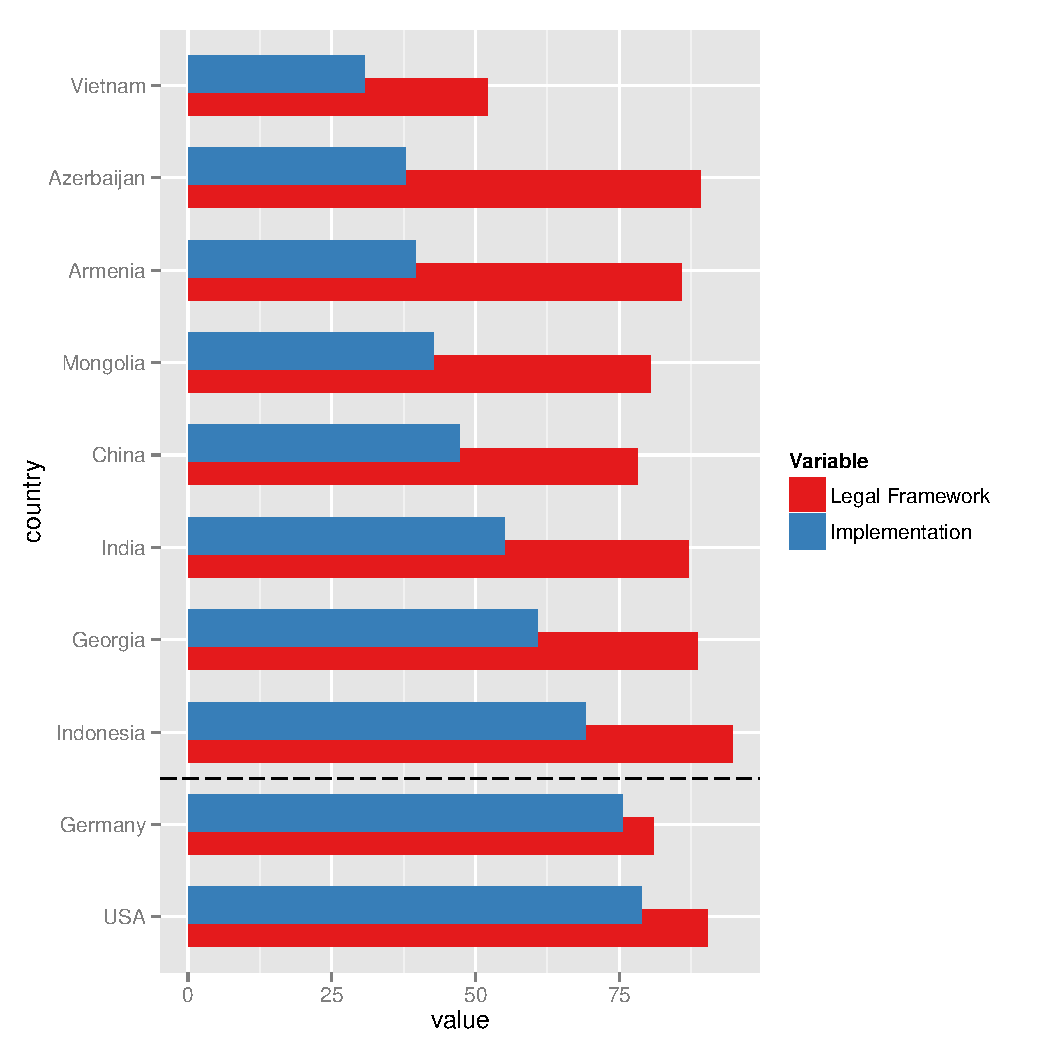
\includegraphics[width=0.9\textwidth]{implementation}
\captionof{figure}[The Severity of Implementation Gap]{The red bars show that most ADB member countries (below the dashed line) already have excellent legal framework, comparable to that of OECD countries (above the dashed line). However, the blue bars show that, in terms of implementation, ADB member countries all rank at the bottom, with the exception of Indonesia as a measured success. Source: \citet{Integrity2012a}. Note: These are all the relevant countries (OECD, ADB members) that are included in the Global Integrity Report.}
\label{fig:implementation}
\end{figure}

But we---as committed organizations and passionate professionals---care not about laws on paper but lives on Earth. Does the experience of corruption improve accordingly? Unfortunately not, as the rate of progress remains glacially slow (Figure \ref{fig:worldcorruption}). Even if we use an optimistic estimate of countries' improvement rate, it will take developing countries hundreds, even thousands of years, in order to catch up with the standard of today Singapore \citep{Pritchett2010}.\footnote{We can estimate the fastest possible improvement rate by assuming that countries had the lowest possible starting point, set to that of Somalia today.} Our relentless effort to promote best practice in institutional form has led to improvement, but only in the sense that a new anti-corruption law passed with little effect is an improvement, and that development finally achieved after hundreds of years is a success.

\begin{figure}
\centering
\animategraphics[autoplay,loop,controls,width=\linewidth]{1}{Rplot}{1}{13}
\captionof{figure}[Corruption in the World, 1996-2011]{The data shows that the pattern of corruption remains stubbornly stable despite over a decade of anti-corruption effort. There is even a deteriorating trend in Asia, reflected by the reddening colors. Source: World Governance Index (WGI). Note: The animation can only be viewed in Adobe Acrobat.}
\label{fig:worldcorruption}
\end{figure}

Of course, that is not to say all forms of technical assistance (TA) and knowledge solution are not valuable. If there is a new drug or construction technology, it should not be held back outside the countries' reach. However, in governance and anti-corruption issues, the centerpiece is people, whose political interests and interactions in each country are complicated and unique. In this setting, transplanting best governance practice is not as straightforward as pouring concrete or combating viruses.

And that is the short answer to why implementation often fails. This paper will provide the more detailed answer, explaining how reform initiatives (both supply and demand sides) erroneously assume a principal-agent framework, in which the state and the citizens are monolithic entities with a single-minded interest in better governance. On the contrary, corruption is, at its core, a collective action problem, caused by the fact that the benefit of bribery and patronage (for \textit{both} the official and the citizen) is immediate and concentrated, whereas the cost of poor governance is dispersed and opaque. Fighting corruption, therefore, is fundamentally about building the political will that rallies the people and reform-minded officials under the promise of change.

Keeping in mind its key message about political will as the prerequisite of reform, this paper is structured accordingly. Section \ref{sec:principalagent} analyzes current governance initiatives, showing that they are driven by a principal-agent, instead of a collective action, framework. This thinking leads to the mistaken belief that the greatest obstacle to reform is a lack of resource and design expertise, both of which are eagerly provided by institutions such as ADB \citep[16]{GlobalIntegrity2012}. Section \ref{sec:collectiveaction} discusses two case studies of Indonesia and Vietnam to emphasize that reform has always been a deeply political, not bureaucratic, matter, and that its success and failure have always depended on building the political will.

Section \ref{sec:currentstrategy} takes a look at ADB's current anti-corruption strategy, pointing out its inattention to the collective action framework. Section \ref{sec:IB} proposes the ``Indicators and Benchmarks'' (IB) as an appropriate strategy for ADB to nurture the political will for reform in a sanitized, politically-neutral manner. By comparing local performances in sectors that have immediate impacts on people's welfare, this strategy rewards reform-minded officials and invigorates the public interest in the cause of anti-corruption.

Lastly, section \ref{sec:conclusion} concludes and emphasizes that this IB strategy is not yet another new tool to directly ``cure'' corruption. Rather, it is a change in mindset, geared towards cultivating an enabling environment for the people to fight against corruption themselves. After all, it is only the people themselves that can, and should, do the strenuous work of shaping their countries' destiny. We must cheer them on, but the journey towards betterment is theirs to travel.

\section{The prevalent principal-agent framework} \label{sec:principalagent}

\subsection{Supply side initiative} \label{sec:supplyside}
Explicitly named or not, our current approach to governance and anti-corruption is deeply wedded to the principal-agent framework. In the supply side approach to governance, the principal is the government, which has the best interest of the country at heart, yet struggles to get the agents (individual bureaucrats and officials) to act accordingly. Given this line of thinking, development agencies have concentrated their efforts on helping the government improve the performance of its agent, both via better capacity development (e.g., modern budget process, staff training, technology) and better monitoring  (e.g. audit, evaluation).

Underlying this framework is the assumption of the government as a monolithic entity with the single-minded goal of improving the people's lives. Yet this assumption is not defensible. The state does not exist---there is only a collective of individual bureaucrats and politicians with their own goals and interests, an all too human one of which is self-enrichment (\citealp{Booth2012}, \citealp{Shleifer2002}). Under the pressure of the development community and in order to keep the stream of aid flowing, politicians may allow the adoption of modern bureaucratic form while keeping the function riddled with opportunities for rent-seeking.

In recent years, it has become increasingly clear that this improvement in form but not in function is in fact happening.  Coining this phenomenon ``institutional mimicry,'' \citet{Andrews2009} points out several reasons why development agencies are successful at influencing governments into adopting the best laws and processes, but much less so at improving the actual practice. Firstly, much of the implementation process is simply not visible to external agencies. Secondly, any attempt to influence an organization's core practice would have an impact upon the material interests of officials, and thus would engender much greater resistance. This leads to a duality of de jure and de facto governance, ubiquitous in public finance, where ``budgets are better made than executed, practice lags behind the creation of processes and laws,'' despite being a core focus of our development agenda \citep{Andrews2010}.

It must be made clear that there is nothing harmful about the adoption of best practice per se. Instead, the key question is whether the government---the principal---is genuinely interested in better managing its agents. If yes, as seen in all development miracles in history, it will automatically look outward for best practices. For example, Meiji Japan tried to copy the best models in the Western world---Britain's postal office, France's police, Prussia's army---and succeeded \citep{Krause2013}. Likewise, in 1980s China, the idea of exposing state-owned enterprizes (SOE) to free market mechanisms came directly from Deng Xiaoping's 1978 visit to the capitalist factories of Japan \citep{Coase2012}. Instances of such unified political will are exceedingly rare---and yet that is the starting assumption of supply side governance initiative.

\subsection{Demand-side initiative} \label{sec:demandside}

The aforementioned shortcoming of supply side initiatives does not escape the attention of development practitioners, arousing an interest in the demand side approach. In this framework, the people are the principal, who struggles to ensure that their government, the agent, works toward their best interests. At first sight, the idea makes great sense: since the government is not necessarily committed to citizens' need, we must empower the citizens to claim their rights with better transparency and accountability.

However, just as the state does not exist, neither does the people---there are only rational individuals weighing the cost and benefit of fighting against corruption. In a thoroughly corrupt system, an individual acting ethically has little impact while giving up the immediate benefit of speedier service or patronage bribe. Therefore, even if the majority in a society utterly condemns corruption, it is not in any individual's interest to stand up and take the fight alone \citep{Persson2010}. In other words, corruption is the result of a \textit{second-order} collective action problem. The society may coordinate to come up with a moral and legal system (first-order problem) that condemns corruption, but no one is willing to incur individual cost to enforce the code (second-order problem) \citep{Heckathorn1989}. This obstacle to enforcement is especially severe at both ends of the spectrum: in very small and traditional societies (such as Pacific countries), where the wrongdoers are often one's own relatives, and in very large societies (such as the Philippines' dispersed population), where the victims are so far removed from one's clique that their plights do not arouse righteous indignation.

As dismaying as it sounds, evidence shows that the people do not always have their collective good as the highest priority. In fact, contrary to the assumptions of the principal-agent framework, voters do not punish corrupt politicians at the poll, seeming to ``display relative indifference to the moral culpability of elected officials'' \citep{Chang2007}. Indonesia's Parliament, widely considered the most corrupt entity in the government, is democratically elected after all \citep{Integrity2012a}. Similarly, the Philippines' patronage politics, rife with vote-buying and grassroots intimidation, has been an intractable character of the country's electoral system for decades \citep{Sidel1999}. Even though it is better for the country to get rid of patronage, no individual voter has the incentive to forgo the canvasser's bribe or to suffer the retaliation. It is egregiously simplistic to think that the citizens will always be the ``principled principal'' and discipline the scoundrel politicians---and yet, and again, this is exactly what the principal-agent framework assumes.

Freeing ourselves from this framework, it is no longer surprising that a host of randomized controlled trials (RCTs) on greater transparency and accountability have produced disappointing outcomes. For example, \citet{Banerjee2010} shows that communities have great difficulties in participating to improve the school system, even when they are provided the information about school performance and have the desire to change it. The culprit is a general skepticism that large group action against school officials is likely to be sustained, thus prompting the citizens not to join the effort in the first place. Similarly, \citet{Olken2005} finds that increasing grass-roots participation in infrastructure project does not reduce corruption, suggesting a free-rider problem as people rely on others to monitor corruption in their stead. In a comprehensive review of all RCT studies concerning transparency and accountability initiatives, \citet{Joshi2010a} shows mixed results in all types of intervention. The emerging conclusion is that success is only possible when the citizens are able to coordinate and impose formal sanctions---otherwise, intervention can only produce short-lived results.

\section{Collective action in action} \label{sec:collectiveaction}

As Section \ref{sec:principalagent} discusses, the issue of corruption does not fit in the principal-agent framework. On the contrary, since the benefit of corruption is concentrated and immediate while the cost is diffused across society, it is a classic collective action problem. Given the cynicism and mistrust that corruption breeds in a society, an individual may rationally ask himself why he should stay clean while his neighbors do not. Why play by the rules when no one is? For this reason, even when the entire society abhors corruption and when the majority is conscientious men, the problem persists in a wretched equilibrium. As a public good, fighting corruption will always suffer from free-riding and be in short supply.

And yet there is hope. The world is not consumed entirely by corruption---the collective action problem does get solved. When talking about successful anti-corruption programs, we often think about the remarkable stories of Singapore and Hong Kong. However, these are highly idiosyncratic cases of small states and strong leadership, which make top-down societal coordination much more feasible. A better source for lessons of nation-wide reform is the past success of today's developed democracies. In 17th century England, unprecedented reforms, leading to the accountability of the King to the Parliament and the Electors, were not good-willed proposals but political tools of the elites to protect their own interests \citep[5]{Johnston2010a}. Similarly, when 19th century American cities were captured by powerful machine bosses,\footnote{Machine bosses held nominal city offices (or none at all) but controlled the patronage system in American cities, often doling out favors to immigrants in exchange for their votes.} the anti-corruption zeal was fueled by bitter political fight between power holders: old political bosses and their immigrant voters versus rising property owners and businessmen, who became disgruntled with increasing graft \citep[204]{Rose-Ackerman1999}.

All of these cases show that reform does not materialize because it is good for the public, but because it is good for a cohesive group with strong enough political power. When the conditions exist for the emergence of such group(s), there is a chance for reform to persevere and succeed. It is worth emphasizing that this kind of tectonic demographic shift takes decades to happen. Recruitment in America's civil service went from 10\% to 80\% meritocratic in 40 years, while its cities alternated between machine boss and legitimate parties throughout the first part of 20th century \citep{Rose-Ackerman1999}.

Do we find the same narrative of reform in Asia today? The tale of two countries, Indonesia and Vietnam, the best and worst performers in \citet{Integrity2012a} report among ADB members, illuminates how the political will remains the fundamental prerequisite of reform.

\subsection{Indonesia's success} \label{sec:Indonesia}

After the fall of President Suharto in 1998, Indonesia underwent major reforms in all aspects of state institutions, including both basic political foundation (the electoral system, an independent judiciary) and bureaucratic reform (a consultative budget process, tighter fiscal rules).

But nothing exemplifies the reform success more than the near 100\% conviction rate of the newly created Corruption Eradication Commission (KPK). Better yet, the Commission accomplished this statistic not by going after only small fish. On the contrary, the KPK has successfully prosecuted senior parliamentarians, bureaucrats, police officials, and powerful businessmen \citep{Schutte2012}.

These reform measures succeeded thanks to a serendipitous convergence of various factors, leading to strong support from both the people and the government. First, during Suharto's rule, a thick network of civil society was allowed to exist. Therefore, at the start of reform, there were already more than 11,100 functioning civil societies, including two largest mass-based Muslim organizations in the world \citep{Harris2011}. These organizations had had years of successful operations, thus facilitating trust and coordination among the people. Second, Indonesian reformers pursued ``accommodative reform,'' i.e. eliciting the political support of old powers by giving them a share in the new pie. For example, while new parties are facilitated, the old party of Suharto was not abolished. The decentralization effort did empower the local governments, but also offered rent-seeking opportunities that appeal to local elites \citep{Hadiz2004}. These were not first-best reforms, but without such compromise any reform would not have been possible at all \citep{Harris2011}.

Despite its success, the KPK remains surrounded by ugly political battles, reminding us that anti-corruption effort encroaches upon the interest of powerful groups that are determined to maintain their stranglehold \citep{Kimura2011}. In 2009, the KPK and the traditional police department attacked each other, leading to a series of arrests against KPK leaders and releases of wiretap evidence against the Chief Detective \citep{Luebke2012}. The KPK also faced great challenge from the Parliament, which, in 2009, tried to restrict the wiretap ability of the KPK and compromise the national corruption court with provincial courts, and in 2011, attempted to reduce the amount of jail time for graft offenders \citep{TransparencyInternational2011}.

Throughout the saga, it was the united stance of Indonesians that played a crucial role in protecting the effectiveness of reform. During the 2009 fight between the KPK and the police department, mass protests in urban centers and virtual domains (1 million online petitions were registered) led to the release of two leading KPK investigators. Even more admirably, the political will has maintained its strong current until today. In 2012, as the Parliament repeatedly stymied the KPK's request for funding, millions of ordinary Indonesians pledged to donate their little money to the agency \citep{Jaaffar2012}. A campaign that urged President Yudhoyono to support the KPK in its investigation of a multibillion rupiah infrastructure project also potentially reached more than 9.4 million internet users \citep{Mahditama2012}.

\subsection{And Vietnam's lack thereof} \label{sec:Vietnam}

Prompted by a 1997 rural unrest in Thai Binh against misuse of infrastructure fund, Vietnam implemented its own ``grassroots democracy'' program as an anti-corruption initiative, epitomizing the demand-side approach sans the vocabulary. The policy includes three prongs of approach: greater transparency (i.e. publishing local budget allocations), greater participation (i.e. incorporating citizens' input in budget planning), and greater monitoring (i.e. allowing citizens to file complaints against local officials).

However, the implementation of this initiative fell flat, attracting little participation from the citizens. The reason lies deep in Vietnam's political landscape, which is marked by the dominance of executive power over the legislative and the judicial branches \citep{Vasavakul2002}. For this reason, people are rightly doubtful about the possibility of sanctioning administrators based on their failure to deliver public services. Furthermore, under the shadow of a strong state, Vietnam's civil society is very weak, with the majority of popular organizations co-opted under the banner of the state-funded Vietnamese Fatherland Front \citep[3]{Thayer2009}. The resulting apathy is hardly surprising---interviews with local people show that, despite the greater opportunities to exercise their democratic rights, the villagers felt concerned only if their personal livelihood was jeopardized. Many commented that they did nothing with regards to corruption because ``nothing would change old ways'' (\citealp[28]{Duong2004}; \citealp{Fritzen2005}).

\section{ADB current strategy} \label{sec:currentstrategy}

As expounded in Section \ref{sec:collectiveaction}, the will for reform is greatly contingent upon the political structure of the country. A reform initiative, one that spans five or even ten years, would not be able to alter the country's power relation or to rebuild its social trust and civil society. This poses a dilemma for the development community: a short-term anti-corruption initiative without indigenous political will cannot work, but a long-term strategy to build the political support for reform is neither practical (given the rapid cycle of loans and projects) nor justifiable (given the messy politics that inevitably ensues).

This difficulty manifests clearly in ADB's anti-corruption effort. To date, there were three TA programs to member countries, including one training program for Nepalese auditors and two programs to assist the aforementioned KPK \citep{ADB2003, ADB2005, ADB2011}.\footnote{Temporary note: Information on more programs with anti-corruption theme are being tallied as it is not always evident from project's description.}  Whereas the short-term technical training successfully provided better staff, technology, and resources to the agencies, it did not address political will, the real bottleneck of implementation gap. In fact, as soon as ADB ventured out of the purely technical area, it encountered tremendous resistance and apathy. For example, despite the enthusiasm and expertise of the consultant team in Indonesia, their advice was largely ignored in the drafting of the KPK's function \citep{ADB2003, Schutte2012}. This experience highlights several difficulties to get involved in a country's political matters. Firstly, it is hard to fit the short time horizon of a project with the indeterminate nature of reform. Secondly, the first-best reform that TA offers is often not viable politically, and thus of little relevance to reformers in the trench.

Besides dedicated anti-corruption projects, under GACAP II, ADB streamlines governance and anti-corruption into all sectoral projects, embodied in the cascading risk assessment and management plan (RAMP). This is a laudable idea---certainly, since all projects involve working with the government on the ground, everyone would do better by keeping governance issues in mind.

However, the impact of this strategy on member countries' corruption is likely to be limited for several reasons. Firstly, in design, the RAMPs only point to weak capacity in the system, which are symptoms, not causes, of corruption \citep[6]{ADB2013}.\footnote{For example, the identified risks in Lao PDR include weak public finance mechanisms, weak capacity, irregularities in procurement, and rising corruption perception \citep{ADB2011a}.} No system materializes and persists out of thin air---rather, it is shaped and maintained by people, and it is the incentive of people that is the ultimate cause of corruption in a country. Therefore, without looking closely at the interests and capability of political actors---the root of the problem---we may be able to trim a rotten branch here and there, but definitely cannot rejuvenate the ailing tree.\footnote{The Philippines Country Partnership Strategy (CPS) includes a political economy analysis, which looks at power holders in the society and root causes of development constraints. This approach is a commendable exception, strongly supported by two internal and two external CPS reviewers (\citealp{ADB2010}, \citealp{ADB2011b}).}

Secondly, in practice, anti-corruption efforts are largely contained at the project level.\footnote{See the example of Nepal in \citet[15]{ADB2013}.} Even if ADB's projects are well safeguarded, these good practices will not automatically propagate throughout the system via demonstration alone. As argued throughout, weakness in a country's system exists because there are beneficiaries that want to keep the system vulnerable, not because its managers do not know any better (and thus can be helped by being shown the best practices). Therefore, whereas the cascading approach does inform the project leaders of the country-level risk, the anti-corruption practice of the projects will \textit{not} necessarily travel upstream to the country level.

\section[Indicators and Benchmarks---a viable strategy]{Indicators and Benchmarks---a viable strategy\footnote{I am intellectually indebted to Prof. Michael Johnston for introducing me to the general IB framework and to Prof. Edmund Malesky for the opportunity to work on Vietnam's Provincial Competitiveness Index---an excellent implementation of this strategy.}}
\label{sec:IB}

What now? We understand clearly that building the political will is instrumental to the success of anti-corruption, yet this matter seems too political for a development agency like ADB to get involved.

Deeply conscious of the tension, this section proposes the use of the \textit{Indicators and Benchmarks} (IB) as a suitable solution. This strategy can solve a political problem while using technical language. It is long-term minded yet can be implemented in quick succession. The crux of the strategy is to measure the governance performance of a country's domestic units (indicators), compare them against one another (benchmarks), publicize the result, and repeat annually. From the demand side, by focusing on issues with an immediate and visible impact upon people's welfare, the strategy can cultivate citizens' interest in reform by demonstrating the potential gains that benefit them directly. From the supply side, by rewarding the high-performing units with recognition, this approach entices officials to join a race to the top. At the foundation of this approach is the acute awareness that relying on public spiritedness alone is not enough. Rather, we must provide and demonstrate the concrete value of reform to each individual, not just to the entire society, in order to tip his cost-benefit balance into joining our cause.

Furthermore, this strategy integrates well with the existing practices and ethos of the ADB. Perhaps the most important advantage is that we can highlight positive achievement rather than accusing of ``corruption,'' a sensitive topic that may shut off governments' cooperation, jeopardizing other projects. Second, the ADB is already proficient in creating a performance index such as this one, which shares many aspects with the Public Expenditure Tracking Survey (PETS) and Community Score Card (CSC). Third, this kind of governance initiative can be broken down into repeated annual exercises, which fit well into rapid loan and evaluation cycles. Fourth, monitoring grassroots governance quality brings ADB closer to its mandate of poverty reduction from macro growth policy or infrastructure development. Fifth, the strategy fits into a growing recognition that composite, cross-national indices, such as Corruption Perception Index (CPI) or World Governance Index (WGI), are too coarse to diagnose any problem beyond saying that there is a problem. For this reason, in its new Governance and Anti-Corruption strategy, the World Bank highlights the advancement of ``actionable governance indicators'' (AGIs). In popular press, \citet{Thomas2013}, Director General of Independent Evaluation, has also opined about the need for disaggregated and locally relevant indicators.  In other parts of the ADB, the South Asia Department (SARD) already moves forward with an index of the same philosophy, comparing trade performance between specific ports, not just countries, in the region (Box \ref{box:tradefacilitation}).

\subsection{Yet another index?} \label{sec:anotherindex}
For a measurement to be useful to policy maker, it must satisfy the following criteria. Highlighted are the most important characteristics to building political will in the IB strategy. As reviewed more extensively in \citet{Pande2013}, while there is no shortage of governance indicators, there is definitely a lack of data that possess these qualities.

\begin{itemize}[noitemsep]
\item{Detailed: whole-country index is too coarse to capture the multiple dimensions of any governance issue.}
\item{Objective: assessment must begin with verifiable evidence, and must be expressed in actual units rather than points on arbitrary scales.}
\item{Noninvasive: the act of measurement must not bias what is being measured, and should not disrupt orderly agency functions.}
\item{Policy-neutral}
\item{Low cost: Since repeated assessments are essential, measurement strategies must be inexpensive.}
\item{Valid and reliable}
\item{\textbf{Transparent and easily understood}: Not only analysts and officials, but citizens and civil society groups, must be able to interpret assessments easily and accurately. The best measurements will the interpretable in terms of positive value.}
\item{\textbf{Trackable over time}: Analysts and officials must be able to demonstrate progress, or lack of it, and successful leaders and managers should be able to claim credit for their accomplishments.}
\item{\textbf{Actionable}: Assessments should not only show that a situation is bad or good, improving or deteriorating, but should also point directly to improvements likely to succeed.}
\end{itemize}

This list is reproduced from \citet{Johnston2010}.

While no single indicator can accomplish all the ideals, this list serves as a backbone for successful IB design.

\subsection{The basic components of IB} \label{sec:basicstrategy}

At its core, the IB strategy is a \textit{repeated} and \textit{publicized} performance audit. Let's say that we collect data on the price that hospital A, B, and C pay for the same kind of standard medical equipment. We find that their expenditures are different: hospital A consistently pays 20\% more than the open market price, hospital B pays about the same, and hospital C manages to pay 10\% less. We conduct similar measurement on other dimensions of performances. We then widely publish the result, visibly commend high performance units, and repeat the exercise annually. As the results accumulate over years, we can focus more on comparing a unit with its past performance rather than with its peers.\footnote{Spearheaded by the U.S. Government Accountability Office (GAO), auditors in developed countries have moved beyond financial audit to performance audit. In Europe, the practice guidelines are maintained by the European Court of Auditors (ECA). The Canadian Comprehensive Auditing Foundation (CCAF) program has also trained 209 fellows from 53 developing countries since 1980 in performance auditing \citep{CPB2010}.}

Good indicators are easy to collect, understand, and compare. Since the IB is unique to each country, we are able to choose key areas with bottlenecks as indicators instead of judging countries against a list of universal criteria for good governance. In order to arouse the interest of the public, indicators must also be directly connected to people's daily welfare. Examples include:
\begin{itemize}[noitemsep]
\item{Expenditure on standard goods, e.g. textbook, school meal, hospital equipment}
\item{Time needed to process routine procedures, e.g. license application}
\item{Quality of infrastructure, e.g. road, electricity}
\end{itemize}

Good benchmarks do not judge units against some ideal standards but take root in the local conditions. The best benchmark is a unit's own past performance, which eliminates all claims of unfair comparison and potential political tension between units. When the data remain thin, there are alternatives, including:
\begin{itemize}[noitemsep]
\item{The norm of performance in other units}
\item{Performance in the private sector (applicable to purchase of basic commodity)}
\item{Statistical model: since a city's infrastructure depends heavily on its initial condition or terrain, multivariate model can take into account these factors and produce an expectation of performance, against which the unit is compared}
\end{itemize}

Two detailed IB examples are discussed later in Box \ref{box:pci} and Box \ref{box:tradefacilitation}.

\begin{textbox}
    \textbf{Box \ref{box:pci}: Vietnam's Provincial Competitiveness Index (PCI)}\\

    \textbf{An understandable, trackable, and actionable indicator.} Initiated in 2005, conducted by Vietnamese Chamber of Commerce and Industry (VCCI) and funded by USAID, the PCI measures governance quality across Vietnam's provinces via business survey, supplemented by hard infrastructure data. The survey asks 9 groups of questions, each pertaining to an important aspect of economic governance as identified by local experts. Examples are: entry cost, access to land, informal charge (corruption), etc.\\

    Examples of individual questions are:
    \begin{itemize}[noitemsep]
       \item{Entry cost: ``How long did it take you to register your business?''}
       \item{Access to land: ``How did you obtain the land that your business sits on?''}
       \item{Regulatory and Administrative Costs: ``From your experience in the province, please list the 3 most troublesome administrative procedures to firms.''}
       \item{Transparency and Participation: ''Please rate your access to these provincial documents and information: 1) provincial budgets, 2) provincial socio-economic development plans, 3) plans for new infrastructure projects, etc.}
    \end{itemize}
    Therefore, the index points to specific bottlenecks in each province's governance. It then repeats this exercise every year to identify and encourage progress.\\

    \textbf{Wide publication to arouse private sector's interest and commend high performers.} Each year, the PCI's launch includes a press conference and the publication of all data on the PCI website. After the first launch in 2005, the PCI team conducted a special report of the index's impact, counting over 145 media reports and four customized provincial diagnostic workshops (up to mid June 2006). In 2012, the annual report dedicated a section on the impact of the PCI on legal reform across provinces, finding that the PCI had been cited in over 60 legal and non-legal documents. To encourage further buy-in, the report highlighted provinces that had been active in this regard.\\

    Anecdotal evidence shows that, despite the risk of survey fatigue, businesses receive the PCI enthusiastically. During an TV news interview in October 2007, a firm owner expressed his frustration with a technical legal issue and commented that he would rate his host province poorly in the next PCI survey. Within a month, local officials responded and resolved the issue. The PCI team shared this anecdote to show that the survey has significant influence on governance quality beyond purely supplying data for research \citep{Malesky2011}.\\

    Source: \citealp{VNCI2005} and other annual reports in the on-going series.
    \caption[An IB example---Vietnam's Provincial Competitiveness Index]{An IB example---Vietnam's Provincial Competitiveness Index (PCI). The PCI uses surveys of domestic and foreign business in Vietnam, supplemented by hard infrastructure data, to assess Vietnam's 64 provinces based on their governance quality.}
    \label{box:pci}
\end{textbox}

\subsection{Anticipating questions} \label{sec:potentialproblem}

\textbf{Why will this work?} This strategy directly addresses the collective action problem of corruption. As discussed earlier, people do not concern themselves with ``good governance'' in and of itself---on the contrary, they are most interested in their immediate likelihood. Therefore, rather than trying in vain to motivate citizens to care about the collective good, this strategy focuses on issues that can be felt privately. Conversely, neither do we idealistically rely on public-spirited officials to take on the fight. We motivate them with public recognition and its associated benefits, such as popularity with voter or professional credentials. No less importantly, the indicators are actionable---they point towards specific problems that allow officials to focus their effort.

\textbf{Is there a risk that officials will game the data?} While this risk can never be fully eliminated, a powerful safeguard is to cross-check the data with the assessment of service users. This has the additional benefit of making sure that we are measuring the relevant indicators. For example, in Vietnam's Provincial Competitiveness Index (Box \ref{box:pci}), the time to acquire a business license reported by the provinces and the businesses is widely different. This is because officials start counting when all the forms are correctly submitted (after which they are required by law to return the license in 5 days), whereas businesses start counting from their first submission \citetext{priv. comm.}. This case shows that the clarity of instruction and speed of feedback is important for businesses, which we would have missed had we relied on official report alone.

\textbf{Will the government cooperate?} Like any governance initiative, this strategy can only be implemented if there is strong support from top leadership. However, this approach does maximize the chance of cooperation by clothing itself in the technical language of fact-finding instead of politically charged topics, such as accountability or citizen empowerment. Furthermore, it does not directly demand the government to change their policies, giving them the respectful space for deliberation and choice. Lastly, if a country depends on attracting FDI or developing the private sector for economic growth, then it is likely to welcome the information that a business survey provides.

As always, gauging the commitment of the government is an important but challenging task. In this case, since the strategy is not the precondition to any financial incentives (e.g. loans, TA), it is at least easier to winnow genuine enthusiasm.

\textbf{Can ADB do this?} In many ways, ADB's existing resource and expertise are already well-suited to this approach. Firstly, the main task of this strategy, i.e. collecting governance data at the micro level, is nothing alien to the development world. A host of micro indicators already exist, including both hard data (e.g. PETS), surveys of stakeholders (e.g. Bangalore's CRC), and a mix of both (e.g. Quantitative Service Delivery Surveys (QSDS), Vietnam's PCI). In addition to efforts by development agencies, the people themselves have sometimes taken the issue of monitoring corruption in their own hands.\footnote{For example, Concerned Citizens of Abra for Good Governance (CCAGG) and Government-Watch (G-WATCH) in the Philippines \citep{ProcurementWatch2008}.}

Secondly, within ADB, there is already the recognition of the need for actionable indicators at the sub-national level. For example, SARD initiated a sub-national trade facilitation index in order to complement existing cross-national databases (e.g. Doing Business, Logistics Performance Index, Enabling Trade Index, Enterprize Survey), which are too coarse to diagnose trade bottlenecks between SASEC (South Asia Sub-regional Economic Cooperation) countries (Box \ref{box:tradefacilitation}).

\begin{textbox}
  \textbf{Box \ref{box:tradefacilitation}: Integrated Trade Facilitation Performance Monitoring (ITFPM)}\\

  \textbf{An understandable, trackable, and actionable indicator.} The ITFPM project is an implementation of the Business Process Analysis (BPA) to document and assess all trade activities along selected transport corridors in SASEC countries. This dedicated database fills the imperative need for detailed information, specific to each port and procedure in the entire supply chain, which cross-national macro indicators do not provide.\\

  \textbf{Data collection method.} The ITFPM demonstrates a wealth of options for governance data collection. Its integrated methodology comprises:
  \begin{itemize}[noitemsep]
    \item{Business Process Analysis (BPA), which interviews relevant stakeholders and covers the whole supply chain before and after the physical movement of cargoes. As a survey, it can collect both objective data (such as number of steps, time, and cost required to complete a business process) and opinion-based data (how information flows among firms and officials).}
     \item{Time Release Studies (TRS), which uses on-site monitoring to zoom in key nodes of the supply chain, i.e. port, airport, border. TRS produces fine-grained, objective data on goods movement through port, e.g. date and time of the arrival, date and time of the beginning of unloading, etc.---all the way to the release and removal of goods.}
     \item{Time-Cost-Distance (TCD), which uses GPS navigators to track the physical movement of cargoes. It then outputs a graphical presentation of the entire transport process, visualizing each procedure or distance (x-axis) and the time or cost it takes (y-axis).}
  \end{itemize}

  \textbf{Sustainability.} Emphasizing the importance of repeated measurement, the ITFPM project develops plans for 1) relying on existing think-tank or research institution with a relevant mandate, 2) capacity building for national and regional experts, and 3) establishing a ``training of trainer'' mechanism.\\

  \textbf{In short, the ITFPM initiative organically embodies key IB components}, even without deliberate design or explicit language. This shows that the IB strategy is not a new fad originating from wishful thought experiments, but an augmented governance measurement that sprouts from the real need of reformers. At the same time, the one difference (at least initially) between the ITFPM and the proposed IB strategy cautions us about a potential hurdle to implementation: countries' officials agree with the project on the condition that data collected by the ITFPM has to be shared selectively among officials and a segment of the private sector. In the long run, the ITFPM does envision a wider engagement, including the Public-Private Partnership, which galvanizes private sector's support by communicating about the benefits of the system and showcasing progress.\\

  Source: \citet{ADB-SARD2013}; Interview with Mr. Cuong Nguyen, Senior Economist, SARD.
  \caption[An IB example---ADB's Integrated Trade Facilitation Performance Monitoring]{An IB example---Integrated Trade Facilitation Performance Monitoring (ITFPM): an initiative by the ADB and the United Nations' Economic and Social Commission for Asia and the Pacific (ESCAP) to profile all trade transactions along selected SASEC transport corridors.}
  \label{box:tradefacilitation}
\end{textbox}

\textbf{What does ADB need to improve?} As discussed above, ADB already has great experience with this type of governance data collection. On the other hand, it needs to invest heavily into its knowledge of a country's political economy. This shift in focus will improve ADB's governance agenda in two ways.

Firstly, it helps ADB identify when TA does work. Throughout the paper, it is argued that TA often fails to work because corruption is not always a principal-agent problem---but sometimes it is. When there is clearly a principal and an agent, for example a central government that genuinely needs its tax agency to collect more revenue, then TA will be wholehearted welcome and implemented. The trick is to identify \textit{genuine} need and interest from the government, which is all the more difficult since TA comes with little financial obligation. A deep understanding of a country's political economy is required to make this diagnosis, as shown in the successful approach of the Cambodian resident mission.\footnote{The Cambodian RM has a checklist of four prerequisites before engaging in any project with the government: 1) Is the problem relevant to ADB's mandate? 2) Is there a real commitment from the government? 3) Can the problem be solved by TA or is it subject to political constraint? 4) Does ADB have the resource to address this problem? \citep{ADB-IED2013}.}

Secondly, with regards to the IB strategy, country knowledge is critical to identify potential point of entry. Who will be our basic constituencies? Everyone is affected by corruption, and thus a potential supporter if not for the fact that the dispersed cost of corruption renders the political will hard to sustain in the first place. Therefore, we must identify potential ``stakeholders who suffer immediate and tangible costs of corruption, and have resources they can mobilize against it.'' Small and medium businesses are promising proponents, for they do have resources beyond subsistence and, unlike large corporations, are likely to be victims rather than accomplices of a corrupt network. Another possibility lies in existing networks, such as religious or communal organizations. In any case, the goal is to ``identify organized segments in a country's social, political, and economic areas, educating people about the costs of corruption while searching for those who find them most oppressive'' \citep[7]{Johnston2002}.

This task requires a deep political economy analysis, which is not yet a staple in ADB's governance and anti-corruption strategy. A commendable first step is RSDD's recent guidance note on how to conduct a political economy analysis. In response to internal reviewers' concern, RSDD promised to put out more detailed operational guidance following the GACAP II implementation review \citep{RSDD-ADB2013}.

One reviewer of RSDD's report also insightfully notes that a country's political economy has a tendency to change very rapidly---``something that may be deemed as unfeasible one month, may become a key reform priority in the next, either because of a change in vested interest groups, an exogenous factor, or a change in politicians themselves'' \citep[reviewers' comments]{ADB-RSDD2013}. This concern about the volatility in political economy is a reason to support ADB's on-going measures to enhance its operations in DMCs via RMs, which are best situated to detect, report, and take advantages of rapid changes in the local political environment. Preliminary findings of an IED's on-going evaluation on ADB's decentralization show that RMs are inadequately equipped with staff strength and decision making power and that the bulk of ADB's skills, activities, and authority remain centralized in HQ. Given RMs' proximity to clients and the potential operational effectiveness and efficiency gains, the draft report recommends that ADB further decentralizes its operations with more staff, functions, and authority delegated to field offices \citep{ADB-IED2013a}.

\section{Conclusion: Change the mindset, not the tool} \label{sec:conclusion}

This paper does not aim to propose yet another new anti-corruption tool, all of which have multiple and unavoidable vulnerabilities to failure. There are simply too many moving parts in any anti-corruption initiative. Factions in the government that fail to strike a deal, bureaucrats that refuse to cooperate, groups of citizen that decide participation is not worth the effort---reasons that corruption exists in the first place---any of them can bring the entire endeavor to an ineffective limbo.

Worse yet, there is little we can do to directly intervene for no one truly knows the \textit{immediate} causes of reform. Everything is obvious, but only after it happens. All reforms and crises can be ``predicted,'' but only \textit{ex post}, when any writer with an average sense of imagination can string together facts and factors into a pattern, a story, a narrative that is hidden in plain (hind-)sight. Indonesia's reform is a prime example---it is a country marred by social and religious cleavages, kept together only by thin history and dispersed geography, consumed by systemic corruption, under the threat of the military in politics---and yet against all odds and prognoses, the country underwent four constitutional amendments, laid a democratic foundation, and put together an anti-corruption agency with force. To be even more humblingly reminded of our ability to plan and predict, we need not look any further than this summer of 2013, when protests against corrupt governments erupted where things had always been business as usual. The Brazilian protest that was sparked by a bus fare hike, the Turkish sit-in against a construction project---they all have trivial starts, the likes of which had been stamped out before. In the dark of night, these are luminous flickers---is this one a firefly, or a spark that will set the field ablaze? It is impossible for us to know.

In other words, we cannot reliably predict how, when, and where collection action will emerge. And thus, unlike the principal-agent problem, the collective action issue cannot be ``solved'' by a direct, definitive, and universal method. For this reason, this paper proposes the IB strategy not as a new tool, but as a different mindset. Instead of implementing a standard drug for all ailing systems, it emphasizes the need for much more diagnostic work, for deep country understanding that identifies strong constituencies of reform. Then, instead of trying to ``solve'' corruption directly, it aspires to build the enabling environment and to nurture the interest of these constituencies in good governance.

In essence, this paper does not argue for the replacement of a universal band-aid with another kind of panacea.  The new mindset recognizes that countries are often stuck in an equilibrium of corruption not out of ignorance or a lack of tools. Thus, as a baseline, there are few things that ADB, whose greatest asset is technical knowledge, can do. Even with the IB strategy, we will not know exactly when and how it will lead to anti-corruption reform. But we do know that this strategy 1) maximizes the possibility of entry by being clothed as technical, 2) provides valuable information regarding grassroots governance in the short term, 4) facilitates collective action in the long term, and 4) fits well with ADB's organizational capability. This may be a small step, but a step and a feasible one nonetheless.

Make no mistake, this is no ``solution'' to corruption, no blazing reform. Only the people themselves can solve their collective action problem, can sweep away moribund trees with their fiery demand. What we \textit{can} do is more akin to a persistent gathering of kindling, while keeping a watchful eye for the right wind, the serendipitous weather. Our job is to build an enabling environment, to cheer on each spark of light. And its very first task is for us to realize that \textit{this} is our right job.

\newpage
\bibliographystyle{chicago}
\bibliography{library}

\end{document} 